\section{Data Warehouse}
The data warehouse design was designed in mind with the Oscar Awards dataset found in Kaggle to analyze the performance of titles over time for business intelligence. 
\begin{figure}[ht]
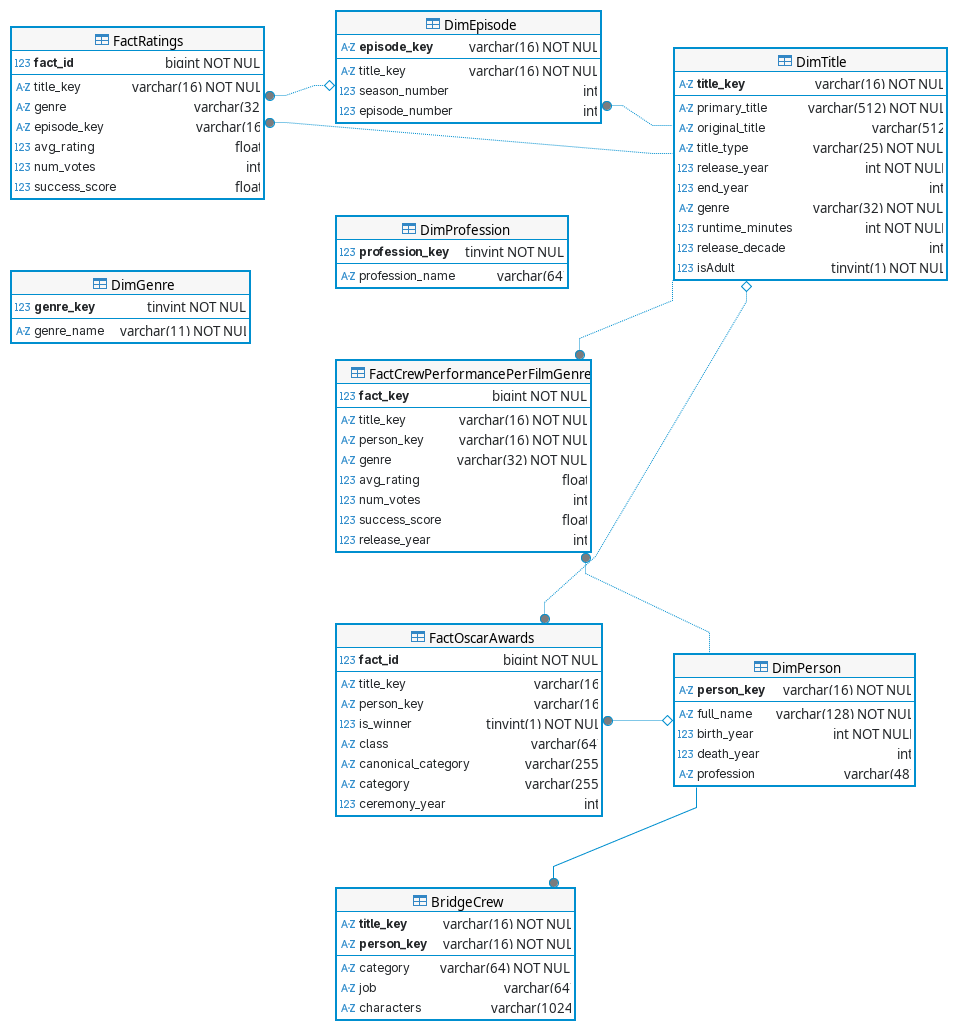
\includegraphics[height=256px, width=256px]{imdb.png}
\caption{Starflake Schema}
\end{figure}

\begin{figure}[ht]
	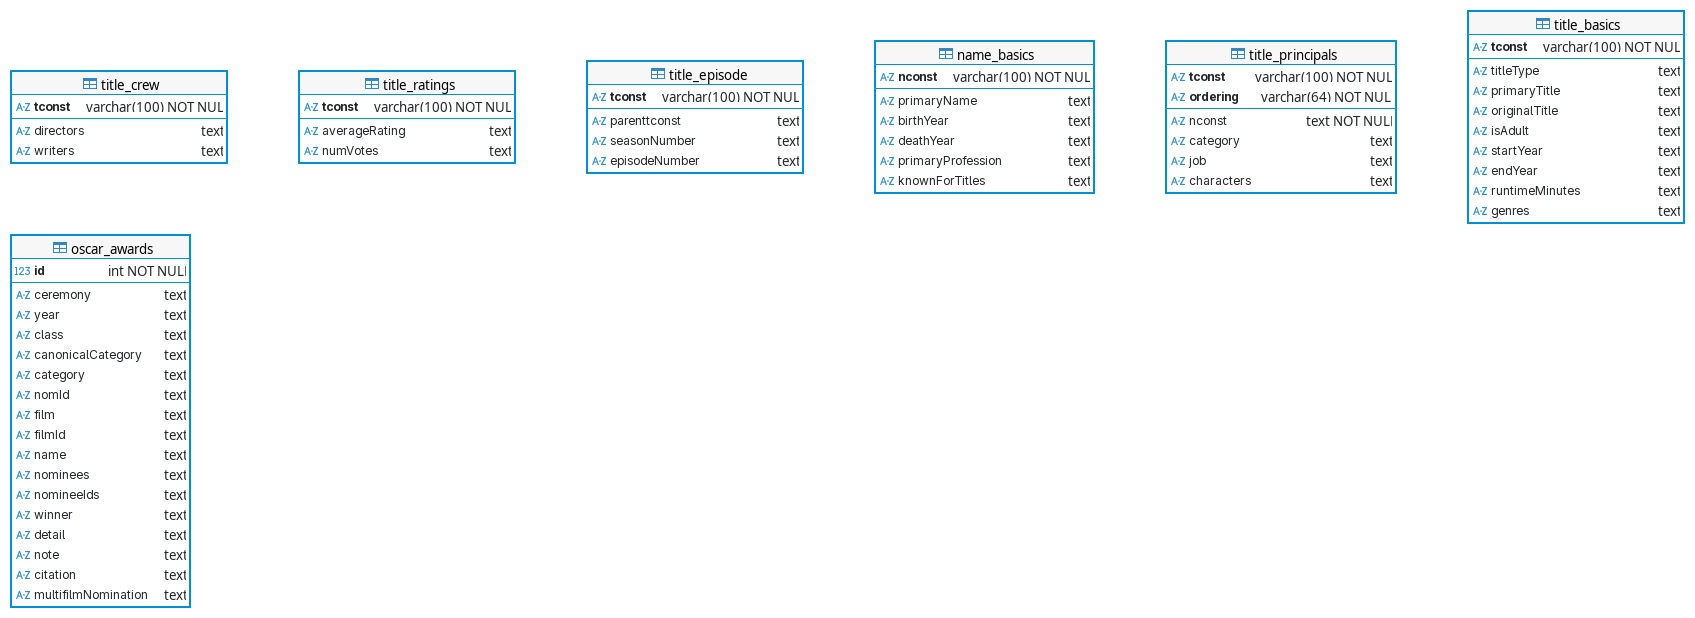
\includegraphics[height=128px,width=256px]{imdb_source.png}
	\caption{Source Schema}
\end{figure}
\subsection{Starflake Schema}
The group decided to use the Starflake schema, a mix of star and snowflake to get the most out of both schemas by having some of the tables denormalized while maintaining a hierarchical structure.  Not only that but the group also factored out the numerous joins required given the number of dimensions the original source dataset has, combining them into a denormalized dimension table became the better option. A good example of this was when the group was deciding on how to tackle genre. Given that the original source data from \textit{title.basics} had a column genre with more than one entry seperated by column if the group uses Star Schema the data will be too bloated while Snowflake Schema will make joins more costly due to requiring a bridge table for Genres to Titles. 
\subsection{Fact Tables}
\subsubsection{Oscar Awards}
To better integrate the Kaggle Dataset for Oscar Awards the group created a fact table \textit{OscarAwards} which is tied to \textit{DimPerson} and DimTitle. The data inside the data set follows the same format of IMDB where the format contains tt and nm followed by a list of numbers for the title and nominee respectively. In the table the data follows columns \textit{canonical\textunderscore category}, \textit{category}, \textit{class} which ties to what category the nominee is involved in where \textit{canonical\textunderscore category} gives the more specific category for their nomination while \textit{class} gives a more broad idea for the category. The \textit{release\textunderscore year} in this table shows the time dimension on when the award was given. 
\subsubsection{Ratings}
On the other hand FactRatings gets the ratings data from the original source which includes the series key and episode key if its a series else it outputs only the film key where episode key is null if its not contained in the episode dimension table. The table includes a one hot encoded genre string which will be explained more in detail in Section \ref{etl}
\subsubsection{Crew Performance Per Film Genre}
Lastly the table FactCrewPerformancePerGenre stores the crew performance given the performance of the film or episode and the entire crew for that film. Each row contains one crew member tied to one film or episode and the rating details from FactRatings. The table also includes a column \textit{success\textunderscore score} while will be explained more in detail in Section \ref{olap}.

\subsection{Dimensions}
In the schema there are six dimension tables, DimEpisode, DimTitle, DimPerson, DimProfession, DimGenre, and BridgeCrew
 
 \subsubsection{Title}
DimTitle stores the title data from the \textit{title.basics} and the year data of each title. 

\begin{center}
$Release Year \rightarrow  Release Decade$
\end{center}

The hierarchy goes from Year to Release Decade where Release Decade is a derived column. The table also stores a one hot encoded version of the genre. Besides this the dimension table also stores the release and end years as well as the titles name and a boolean to know if its an adult film or not. The purpose of having all these is to support Slice and Dice operations.

\subsubsection{Episode}
DimEpisode stores the episode data containing the season number and episode number as the hierarchy. 
\begin{center}
	$Title \rightarrow SeasonNumber \rightarrow EpisodeNumber$
\end{center}


\subsubsection{Person}
DimPerson contains the full name of the person, birth year and a death year if its included. The DimPerson table also includes a one hot encoded version of the profession given that it is possible for the person to have more than 1 profession.

\subsubsection{Genre}
DimGenre is a lookup table that contains the indexes and name of the genre for the one hot encoded genre in the previous tables. The main reason the group decided to stick to one hot encoding was because it became easier to store the genres given a title since the original dataset gave a list of genres per title. 

\subsubsection{Professions}
DimProfession is a lookup table that contains the indexes and name of the profession as well.
The same reasoning applies to the one hot encoded version of professions due to it being easier to read and analyze a one hot encoded string rather than a string seperated by comma for the professions.

\subsubsection{Crew}
BridgeCrew contains the category type of job and the job of the person given the title. The dimension table also has an optional characters field given that the person was an actor for that title. This table also includes the hierarchy of category and job as followed where category is the job category and job being the specific role.
\begin{center}
	$Category \rightarrow Job$
\end{center}

\subsection{Issues Encountered}
\subsubsection{Denormalizing Genre and Profession}
One of the original issues that was addressed by the one hot encoding were the constant fields that could be one hot encoded such as genre and professions since all it takes is to check whether or not the title applies it. This is because if the group converts it to bridge tables for professions and crews respectively the cost of doing joins will be too high. Besides this the group created functions in MySQL to convert the input genres seeprated by comma to one hot encoded data. 
\newline

\subsubsection{Many to Many Relationships}
During the ETL one of the problems that the group encountered was converting data from lists from the original dataset to multiple rows. For example to convert the directors and writers from title crews to BridgeCrew the group had to flatten the strings and map it out to rows. To solve this problem the group decided to use a recursive common table expression to map out the dataset to BridgeCrew. 
\newline


